\documentclass[conference]{IEEEtran}
\IEEEoverridecommandlockouts
% The preceding line is only needed to identify funding in the first footnote. If that is unneeded, please comment it out.
\usepackage{cite}
\usepackage{amsmath,amssymb,amsfonts}
\usepackage{algorithmic}
\usepackage{graphicx}
\usepackage{textcomp}
\usepackage{xcolor}

% % % Packages Added by Louis % % %
\usepackage{comment}
\usepackage{subfigure}
\usepackage{tabularx}
\usepackage[flushleft]{threeparttable}
\usepackage{rotating}
\usepackage{lscape} 
%\usepackage[colorlinks=true, allcolors=black]{hyperref}
\usepackage{pgfplots, pgfplotstable}
\usepackage{tikz}
\usetikzlibrary{trees}
\usetikzlibrary{snakes,arrows,shapes}
\usepackage{listings}
\definecolor{lightgray}{rgb}{0.95, 0.95, 0.95}
\definecolor{darkgray}{rgb}{0.4, 0.4, 0.4}
\definecolor{purple}{rgb}{0.65, 0.12, 0.82}
\definecolor{ocherCode}{rgb}{1, 0.5, 0} % #FF7F00 -> rgb(239, 169, 0)
\definecolor{blueCode}{rgb}{0, 0, 0.93} % #0000EE -> rgb(0, 0, 238)
\definecolor{greenCode}{rgb}{0, 0.6, 0} % #009900 -> rgb(0, 153, 0) 

\usepackage[ruled]{algorithm2e}
\usepackage{multirow}
\usepackage{setspace}
\usepackage{todonotes}
\usepackage{amsmath}
\usepackage{booktabs}
\usepackage{siunitx}
\sisetup{per=slash, load=abbr}
\usepackage{calc}
\usepackage{array}
\usepackage{caption}
\usepackage{url}
\usepackage{pgf}
\usepackage{mdwlist}
\usepackage{graphicx}
\usepackage{epsfig}
\usepackage{dot2texi}
\usepackage{graphicx,stfloats}
\usepackage{graphicx,epstopdf}
\epstopdfsetup{update}
\usepackage{enumerate}
% % % Packages Add by Louis % % % 

\def\BibTeX{{\rm B\kern-.05em{\sc i\kern-.025em b}\kern-.08em
    T\kern-.1667em\lower.7ex\hbox{E}\kern-.125emX}}
\begin{document}

\title{A High-Performance FPGA Accelerator Framework \\for Linear Time-Multiplexed Overlays\\
%{\footnotesize \textsuperscript{*}Note: Sub-titles are not captured in Xplore and
%should not be used}
%\thanks{Identify applicable funding agency here. If none, delete this.}
}

\begin{comment}
\author{\IEEEauthorblockN{1\textsuperscript{st} Given Name Surname}
\IEEEauthorblockA{\textit{dept. name of organization (of Aff.)} \\
\textit{name of organization (of Aff.)}\\
City, Country \\
email address}
\and
\IEEEauthorblockN{2\textsuperscript{nd} Given Name Surname}
\IEEEauthorblockA{\textit{dept. name of organization (of Aff.)} \\
\textit{name of organization (of Aff.)}\\
City, Country \\
email address}
\and
\IEEEauthorblockN{3\textsuperscript{rd} Given Name Surname}
\IEEEauthorblockA{\textit{dept. name of organization (of Aff.)} \\
\textit{name of organization (of Aff.)}\\
City, Country \\
email address}
\and
\IEEEauthorblockN{4\textsuperscript{th} Given Name Surname}
\IEEEauthorblockA{\textit{dept. name of organization (of Aff.)} \\
\textit{name of organization (of Aff.)}\\
City, Country \\
email address}
\and
\IEEEauthorblockN{5\textsuperscript{th} Given Name Surname}
\IEEEauthorblockA{\textit{dept. name of organization (of Aff.)} \\
\textit{name of organization (of Aff.)}\\
City, Country \\
email address}
\and
\IEEEauthorblockN{6\textsuperscript{th} Given Name Surname}
\IEEEauthorblockA{\textit{dept. name of organization (of Aff.)} \\
\textit{name of organization (of Aff.)}\\
City, Country \\
email address}
}
\end{comment}

\maketitle

\begin{abstract}
Coarse-grained FPGA overlays have shown promising advantages such as software-like programmability and fast compilation to improve the design productivity. 
However, few of the existing overlays have been developed as complete accelerator systems, suitable for real-world applications. 
To address this issue, a high-performance overlay system framework is proposed, based on two different memory interfaces, AXI and PCIe. 
We implement these hardware accelerators on ZedBoard (AXI-based) and VC707 (PCIe-based) platforms respectively, and evaluate their throughput and resource usage for a range of benchmarks. 
The proposed AXI-Xillybus-Overlay system achieves a much more area efficient implementation in comparison with a state-of-art time-multiplexed (TM) overlay, referred to as VectorBlox MXP, at the cost of around 50\% of the throughput which is limited by the 32-bit AXI-ACP interface used by AXI-Xillybus compared to the full 64-bit AXI-HP interface used by VectorBlox MXP. 
The proposed DyRACT-Overlay system shows the highest performance among all the proposed overlay accelerators (18\% higher than RIFFA-Overlay, 4.3$\times$ higher than PCIe-Xillybus-Overlay, and 6.8$\times$ better than AXI-Xillybus-Overlay). 
\end{abstract}

\begin{IEEEkeywords}
FPGA overlay, memory interface, framework
\end{IEEEkeywords}

\section{Introduction}
Coarse-grained overlays, implemented on top of the conventional fine-grained FPGA, represent a promising solution to the design productivity problem seen in modern FPGA design. This is because coarse-grained architectures enable faster compilation and software-like programmability, compared to the existing fine-grained FPGAs.  
FPGA overlays can be broadly categorised as spatially configured (SC) or multiplexed. In an SC overlay, a functional unit (FU) is allocated to a single computational operation of the kernel to be accelerated, with FUs connected by a routing network which is essentially static during kernel execution. A multiplexed overlay, on the other hand, shares both the FUs and the interconnect across kernel operations.
A linear time-multiplexed (TM) overlay~\cite{li2016area} has shown potential for use as an area efficient FPGA accelerator, and significant improvements to the architecture were described in~\cite{li2018time} which further improved the overlay performance. 
The streaming architecture based on feed-forward pipelined datapaths allows for a simple linear interconnect of lightweight functional units, thus minimizing the interconnect requirements. 
However, to demonstrate the suitability of the overlay as an FPGA accelerator, it is important to develop a complete accelerator system, with an interface between the processor/memory subsystems and the overlay which is able to provide high-bandwidth (and large scale) data transmission.
An examination of existing FPGA solutions for memory interfaces, showed that most fall into one of two categories, AXI bus-based solutions for FPGA SoC systems (like in Xilinx Zynq) and PCle-based solutions for stand-alone systems connected to a host CPU. 
Among the various frameworks, some of them abstract the interfaces with simple FIFO connections and provide streaming data transfers, which matches the requirements of our proposed linear TM overlay. 

In this paper, we implement accelerator solutions for Zynq-based FPGA systems using the AXI interface and for standalone FPGA systems with PCIe connectivity, based on the Xillybus~\cite{xillybus2018}, RIFFA~\cite{jacobsen2015riffa} and DyRACT~\cite{vipin2014dyract} communication frameworks. 
The architecture of the linear TM overlay and the its essential control circuit are presented in detail. 
We examine the compulsary components for a full working implementation and propose our framework of overlay accelerator integrated with a memory subsystem. 
A detailed description of the programming model for DyRACT-Overlay is presented, which makes it very promising for practical usage.
We evaluate the performance of the proposed AXI bus-based and PCIe-based overlay accelerators for a range of benchmarks. 
The proposed AXI bus-based accelerator is compared to a state-of-art TM overlay referred to as VectorBlox MXP~\cite{severance2013embedded}, in terms of throughput and resource usage. 
We compare the PCIe-based implementations, i.e. PCIe-Xillybus-Overlay, RIFFA-Overlay and DyRACT-Overlay, in terms of throughput and area utilization. 
The DyRACT-Overlay framework is open-source for future research and it is available at https://github.com/louislxw/linear\_tm\_overlay. 


\begin{comment}
The main contributions can be summarized as follows:

\begin{itemize}
\item	
Examine memory interfaces for hardware accelerators implemented on FPGAs, and provide a comprehensive analysis of two of the state-of-the-art integration frameworks, i.e. Xillybus and RIFFA. 

\item
Propose complete hardware accelerator systems by integrating the linear TM overlays with Xillybus and RIFFA interfaces, respectively, and evaluate the throughput and resource usage of these hardware accelerators for a range of benchmarks.

\item
Make comparisons with a state-of-the-art TM overlay, namely VectorBlox MXP, which shows that the proposed overlay achieves approximately 50\% of the throughput, but uses just half of the bandwidth and less than 20\% hardware resource compared to MXP.

\end{itemize}
\end{comment}

\section{Related Work}
%Two of the more common solutions for interfacing FPGA based hardware accelerators are AXI bus-based solutions~\cite{vipin2014zycap, sadri2013energy, xillybus2018} for FPGA SoC systems (like in Xilinx Zynq) and PCle-based solutions~\cite{xillybus2018, vipin2014dyract, gong2014efficient, de2016fflink, jacobsen2015riffa} for stand-alone systems connected to a host CPU. 

%Typical PCIe-based solutions for interfacing FPGA based hardware accelerators can be found from~\cite{xillybus2018, vipin2014dyract, gong2014efficient, de2016fflink, jacobsen2015riffa}. Most of them achieves high bandwidth close to theoretical maximum.  

\subsection{Time-Multiplexed Overlays}

ADRES~\cite{mei2003adres} appeared to be the first integration of a very long instruction word (VLIW) processor tightly-coupled with a coarse-grained reconfigurable matrix. 
Some of the functional units (FUs) and register files (RFs) are shared by the VLIW processor and the reconfigurable matrix. 
Thus, there is no need to transfer the data between the processor and the reconfigurable array compared to the tranditional CGRAs. 
Taras~\cite{taras2019impact} implemented the ADRES as overlays on Intel and Xilinx FPGAs using CGRA-ME modeling framework~\cite{chin2017cgra}. 
The ADRES overlay can achieve up to $1.6\times$ speedup on Fmax and a reduction of 41\% LUT usage, with the FPGA architecture optimizations. 


QuickDough~\cite{liu2015quickdough} was proposed to address FPGA design productivity issues. 
It is comprised of an array of nearest neighbor interconnected processing elements (PEs), referred to as SCGRA overlay.  
Application specific SCGRA overlay were implemented on Zynq, achieving a speedup of up to $9\times$ compared to the same application qunning on the Zynq ARM processor. 
The 250 MHz FU consists of an ALUm multiport data memory ($256\times$32 bits) and customizable depth instruction ROM (Supporting 72-bit instructions) resulting in significant BRAM utilization. 
Due to the excessive usage of BRAMs, it has limited scalability as a maximum implementation of $5\times$5 array can fit on Zynq, despite of the frequency degradation caused by the tight placement and route. 


VectorBlox MXP~\cite{severance2013embedded} is a commercial soft vector processor overlay targetting Altera or Xilinx FPGAs via the Avalon or AXI interfaces. 
Data transfer is handled by a double-buffered vector scratchpad and a dedicated DMA engine communicating with the scalar host processor via the AXI HP port. 
MXP can operate at a maximum frequency of 110 MHz on a Xilinx XC7Z020 device with 16 vector lanes. 
It demonstrates up to $1000\times$ speedup over MicroBlaze. 
The programming model is user-friendly as it is a combination of ANSI-C and VectorBlox C extensions.  
However, it is difficult to implement the applications which cannot be easily vectorized. 


\subsection{PCIe-based Interface Solutions} 
Northwest Logic~\cite{nwlogic2018} and Xillybus~\cite{xillybus2018} are two representative commercial solutions which support PCIe interfaces for different generations while providing portability across different FPGA devices. 
Northwest Logic is licensed closed source while Xillybus is provided free of charge for research and teaching purposes. 
Xillybus users have full access to customize the complete Xillybus project, including the hardware design, the device driver and the software applications, with good documentation provided.
The latest version (Revision XL) of Xillybus  can achieve a maximum data rate of around 3.5 GB/s for Gen2x8 and Gen3x4 PCIe interfaces.

In addition to these commercial solutions, there are a number of academic PCIe-based solutions, such as DyRACT~\cite{vipin2014dyract} and EPEE~\cite{gong2014efficient}.
DyRACT mainly focuses on dynamic partial reconfiguration over the PCIe Gen2x4 interface, along with a configuration controller and clock management, while EPEE was developed as a general purpose PCIe communication library, targeting a wide range of FPGA devices. 

RIFFA~\cite{jacobsen2015riffa} is an open source reusable framework for the integration of FPGA accelerators with workstations supporting PCIe Gen 2 and Gen3 protocols. 
A scatter-gather DMA-based design bridges the vendor-specific PCIe Endpoint core and multiple communication channels for user defined IP cores. 
The latest release of RIFFA (version 2.2.2) achieves a unidirectional maximum bandwidth of 3.6 GB/s for the Gen2x8 configuration on the Xilinx VC707 platform and 3.5 GB/s for the Gen3x4 configuration on the Terasic DE5-Net.

Other recent solutions include ffLink~\cite{de2016fflink} and JetStream~\cite{vesper2016jetstream}. 
ffLink is an open source PCIe Gen3x8 interface which achieves a throughput of 7.06 GB/s on a Xilinx VC709 platform. 
ffLink is based on the AXI infrastructure with Xilinx CDMA engines, limiting its use beyond Xilinx devices. 
JetStream~\cite{vesper2016jetstream} provides both FPGA-to-Host and FPGA-to-FPGA communication, and supports PCIe Gen3x8  with a peak unidirectional bandwidth of 7.05 GB/s. 
However, poor documentation and tool compatibility issues limit its use.

%Table~\ref{theo_bw} shows the theoretical bandwidth of the AXI and PCIe memory interfaces. 
%Although the total theoretical bandwidth of an AXI interface is comparable to that of a PCIe interface, many of the AXI-based solutions are not able to make full use of all available high performance HP/ACP ports, while the PCIe-based counterparts can support up to 8 lanes and some of them achieve a bandwidth which is close to the theoretical maximum. 
Though TM overlays have shown great potential to impove the FPGA design productivity, few of them have been developed as full accelerator systems except for the existing work investivated above. 
The PCIe-based memory soluctions provides a perfect bridge between the host processor and the FPGA-based accelerators, for their high bandwidth and low latency. 
Among the existing implementations, Xillybus, RIFFA, and DyRACT appear to be the most promising solutions due to their availability, ease-of-use and portability. 
In subsequent sections we develop high performance overlay-based accelerators designs using these solutions and then compare their performance and area overhead.


\begin{comment}
\begin{table}[tb]
	%	\renewcommand{\arraystretch}{1.2}
	\caption{Theoretical bandwidth of typical memory interfaces.}
	\label{theo_bw}
	\centering
%	\small
	\resizebox{\columnwidth}{!}{
		\begin{threeparttable}
			\begin{tabular}{lrrrcr}
				\toprule
				Interface & Frequency & Upstream BW & Downstream BW & Ports/Lanes & Total BW\tnote{1} \\ \midrule
				AXI HP    &   150 MHz &   1200 MB/s &     1200 MB/s &      4      &         9600 MB/s \\
				AXI ACP   &   150 MHz &   1200 MB/s &     1200 MB/s &      1      &         2400 MB/s \\
				PCIe Gen2 &   250 MHz &    500 MB/s &      500 MB/s &      8      &         8000 MB/s \\
				PCIe Gen3 &   250 MHz &    984 MB/s &      984 MB/s &      8      &        15800 MB/s \\ \bottomrule
			\end{tabular} 
			\begin{tablenotes}
				\item[1] In a streaming interface, the throughput is limited by either the upstream or downstream BW, depending on the number of inputs or outputs, and so the maximum theoretical throughput would be half of the total bandwidth reported here.
			\end{tablenotes}
		\end{threeparttable}
	}
\end{table}
\end{comment}
\section{Linear TM Overlay}
\label{section_3}
\subsection{Architecture Description}
We consider a linear array of FUs as a time-multiplexed (TM) overlay similar to the design in~\cite{li2018time} where each FU can be time multiplexed among operations present in a single scheduling stage of a directed acyclic graph (DAG). 
The 32-bit linear TM overlay is comprised of a quasi-streaming data interface made up of two FIFO channels implemented using Block RAMs, which transmit data through daisy-chained fully pipelined time-multiplexed FUs, as shown in Figure~\ref{overlay}. 
By eliminating the fully flexible routability of CGRA-like overlays, this structure achieves a much more area-efficient design, using fewer than 6\% of the logic and DSP resources on a Xilinx Zynq device. 
The initiation interval (II) can be significantly reduced by making minor architectural enhancements, such as adding a rotating register file and replicating the data stream. 
These changes result in a peak throughput of 1.8 GOPS running at a frequency of 335 MHz. %\todo[inline]{Need to clarify based on what frequency of operation?} 
Adding write-back capabilities to the FU design reduces the overlay depth requirement by allowing multiple nodes on the critical path to be combined. 
This also eliminates the need to reconfigure the overlay whenever the application kernel changes, making the overlay suitable for more general purpose applications. 


\begin{figure}
    \centering
	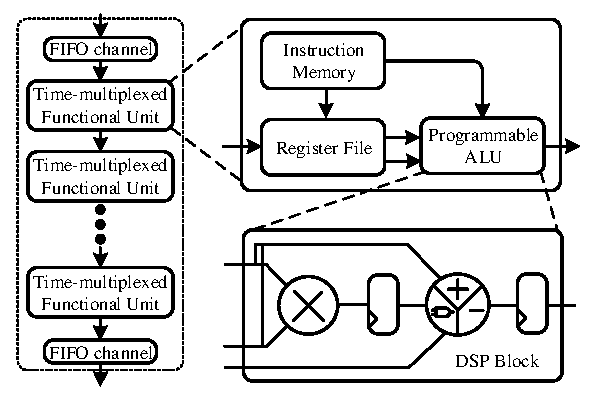
\includegraphics[width=\columnwidth]{Figures/overlay.pdf}
	\caption{A linear TM overlay.}
	\label{overlay}
\end{figure}


\subsection{Overlay Control}
A back-pressure control circuit is built around the input FIFO channel to manage the functionality of the overlay, as shown in Figure~\ref{back_pressure}. 
There are three control signals which indicate the duration for instruction load, overlay setup and data write respectively, referred to as \textit{inst\_load}, \textit{reg\_wren}, and \textit{data\_wren} respectively. 
Initially, FU instructions are read from the memory and streamed through the daisy-chained FUs. 
During instruction load (when \textit{inst\_load} is asserted), both the write enable port of the FIFO and the valid signal (\textit{valid\_out}) for the data output are disabled. 
After instruction load, two integers are written to the back-pressure control circuit. 
The first represents the number of data words to be input to the first FU for a specific compute kernel while the other is equal to the II minus one (II$-1$) and determines the interval between data loads. 
These values are written into the controller when the \textit{reg\_wren} signal is asserted.
%The process of instruction load and overlay setup represent the initialization of the overlay.

The dashed box on the left of Figure~\ref{back_pressure} represents the control module for the write enable port of the FIFO, while the dashed box on the right contains the logic to control the read enable port of the FIFO. 
Data is written into the FIFO when \textit{wr\_en} is high.
The read enable signal (\textit{rd\_en}) for the FIFO is generated from a counter which determines the number of cycles needed to load input data into the FU. 
The counter starts counting from 0 when the \textit{empty} signal goes low (indicating that data is available in the FIFO). The counter counts up until the count value equals II$-1$, at which point it rolls over back to zero.   
The \textit{rd\_en} signal is valid only while the counter is less than the initial number loaded into the back-pressure circuit, limiting the amount of data to be loaded into the first FU.
Once the counter value is greater than or equal to the data load number (in the back-pressure circuit), the \textit{rd\_en} signal is forced low and the input data is buffered in the FIFO.


\begin{figure}
	\centering
	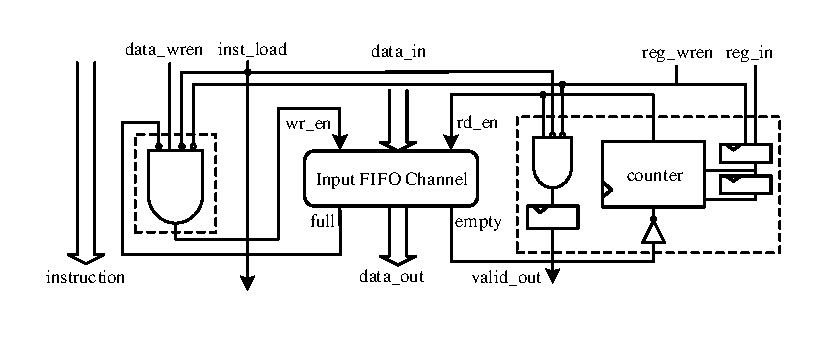
\includegraphics[width=\columnwidth]{Figures/control.pdf}
	\caption{Back-pressure control circuit.}
	\label{back_pressure}
\end{figure}
	

\subsection{Complete Overlay Accelerator Framework}
The linear TM overlay has shown its advantages to implement an area efficient design with fast context switching and high throughput. 
However, to demonstrate the suitability of the overlay as an FPGA accelerator, it is important to develop an interface between the main processor/memory subsystem and the overlay which is able to provide high-bandwidth data transmission. 
As discussed in the previous section, two stream interfaces are required for transmitting the data between the host processor and the overlay accelerator. 
Additionally, it is necessary to set up memory arrays or registers so that the user has access to control the overlay system, i.e. the instruction load, overlay setup, and data write. 


\section{Overlay Accelerator Framework}
A block diagram of the proposed overlay accelerator system, based on an array of linear TM overlays as described in the previous section, which supports both Zynq-based SoC and standalone PCIe accelerators, is shown in Figure~\ref{system}. 
The FPGA memory subsystem provides the interface between the overlay on the FPGA fabric and the ARM processor on a Zynq SoC via the AXI bus (or directly to the memory via the PCIe link). 
For the AXI bus-based overlay, two 32-bit FIFOs are used to connect a single 32-bit linear TM overlay with the memory subsystem. 
%For the PCIe-based overlay, four 32-bit linear TM overlays are used to make full use of the 128-bit data bandwidth and thus reduce the II to a quarter of that of a single overlay. 
For the PCIe-based overlay, we propose replicating four 32-bit linear TM overlays to make full use of the 128-bit data bandwidth. The four overlay instances can implement multiple compute kernels at runtime and thus reduce the II to a quarter of that of a single overlay. 
Data transfers between the internal memory subsystem, the DDR SDRAM and the offchip DRAM are under the control of a scatter-gather DMA engine. 
%The overlays are connected to the memory subsystem via two 128-bit FIFOs. 

\begin{figure}[tb]
	\centering
	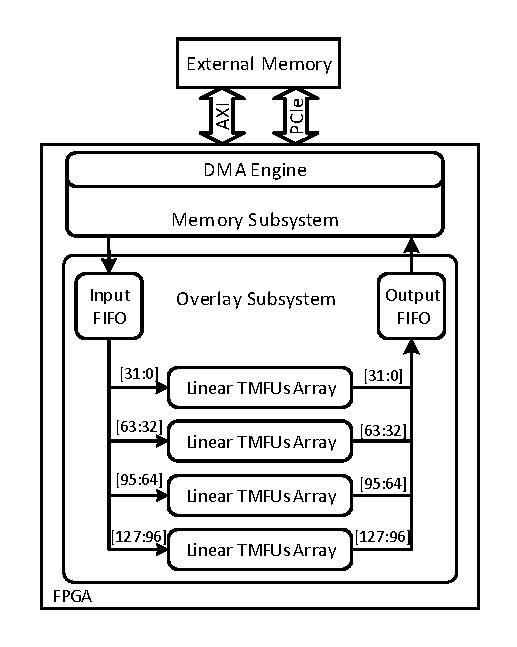
\includegraphics[width=\columnwidth]{Figures/system_new.pdf}
	\caption{The proposed overlay accelerator system.}
	\label{system}
\end{figure}

%\begin{figure}
%	\centering
%	\subfigure[Block diagram of the system]{
%	\centering
%	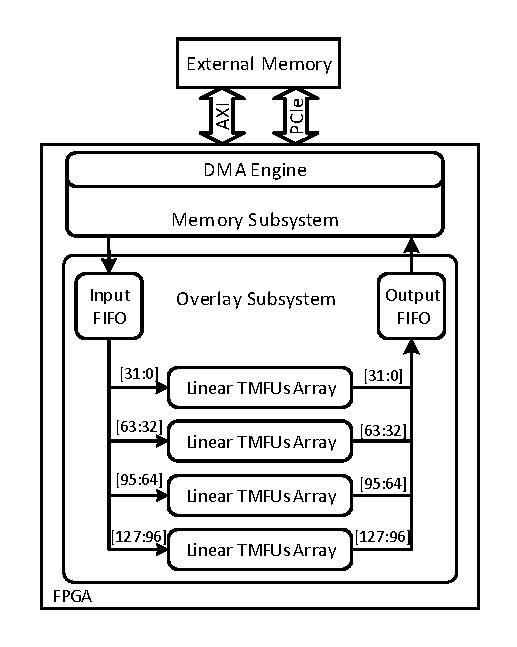
\includegraphics[width=0.9\columnwidth]{Figures/system_new.pdf}
%	\label{a}
%	}
%	~
%	\subfigure[A linear TM overlay]{
%	\centering
%	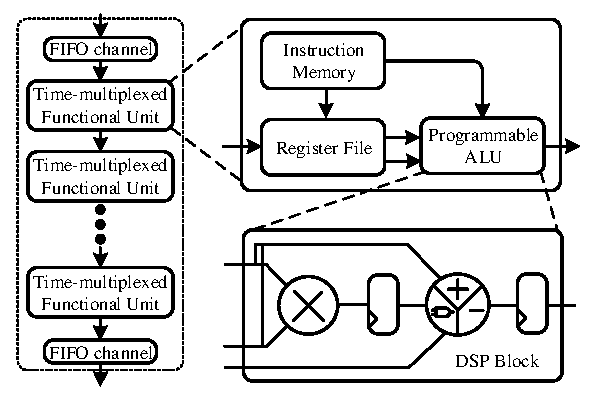
\includegraphics[width=0.9\columnwidth]{Figures/overlay.pdf}
%	\label{b}
%	}
%	\caption{The proposed overlay accelerator system.}
%	\label{system} %% label for entire figure
%\end{figure}


\subsection{Interfacing with Xillybus}
Xillybus is a portable, easy to use DMA-based data transfer solution which provides a simple abstraction of the AXI/PCIe interfaces. 
%There is no prerequisite for knowledge of the AXI or PCIe protocols as all the low-level design is packaged into an IP core. 
One side of the Xillybus IP core is connected to the host processor, while the other side communicates with one standard FIFO, providing six signals to control the data flow. 
%, as shown in Figure~\ref{xillybus}. 
The host processor can be either the ARM processor of the Xilinx Zynq SoC (AXI-Xillybus: for an AXI bus-based solution) or a PC based x86 CPU (PCIe-Xillybus: for a PCIe-based solution). 
Xillybus provides a simple data loopback demo design, along with its driver for the default device files and the software code for testing purpose. 
%After the driver installation and the FPGA is programmed by the Xillybus bitstream, several device files are generated by the host driver which can be read from and written to like any file using basic Linux commands such as \textit{write} and \textit{read}. 
%Users have access to customize the Xillybus IP core by changing the number of device files, their streaming directions and data widths. 
When connecting Xillybus to the linear TM overlay, two standard FIFOs need be used to buffer the input/output data. 


%\begin{figure}[tb]
%	\centering
%	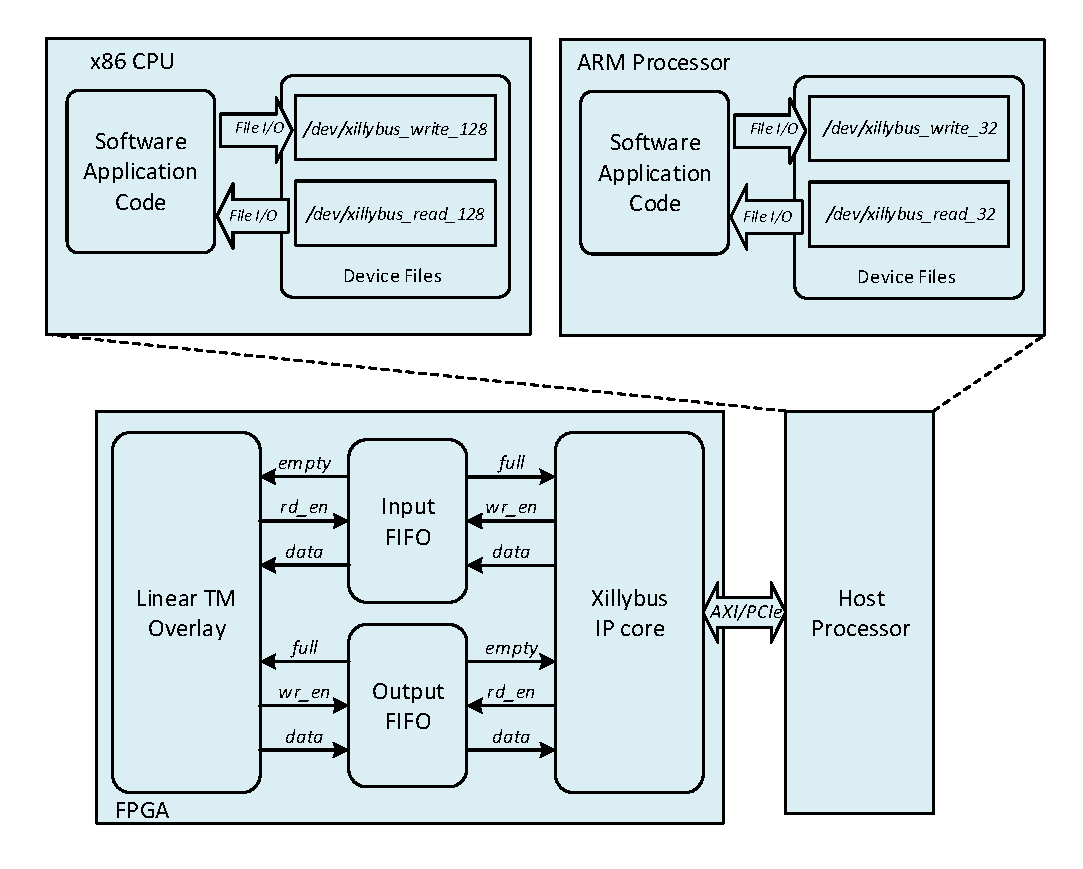
\includegraphics[width=0.9\columnwidth]{Figures/xillybus.pdf}
%	\caption{Xillybus-based overlay accelerator.}
%	\label{xillybus} 
%\end{figure}


\subsection{Interfacing with RIFFA}
RIFFA has a more complicated framework which generally consists of three layers. 
%, as shown in Figure~\ref{riffa}. 
%It can be visually divided into two part, one part containing the device driver and the software APIs in the PC while the other one including all the PCIe hardware interface design in the FPGA. 
%A vendor-specific PCIe endpoint bridges the connection between RIFFA and host CPU via the PCIe link. 
%It is mainly comprised of three layers. 
On the bottom layer, an RX engine and a TX engine are connected to the vendor-specific PCIe Endpoint IP core, which bridges the connection between RIFFA and the host CPU. 
The middle layer supports up to 12 channels which send packets to the TX engine and receive packets from the RX engine through a scatter-gather DMA engine. 
The overlay which connects to the RX/TX FIFOs from the communication channels, is located on the top layer. 
An example design of one channel for data transfer, along with driver and software code, is provided. 
%Dedicated software APIs (\textit{fpga\_send} and \textit{fpga\_recv}) were developed as blocking functions.
Integration of the linear TM overlay with RIFFA is quite similar to that of Xillybus, except
that the standard FIFOs are replaced with first word fall through (FWFT) FIFOs to meet the timing closure. 
%For a more complicated design, multiple channels (up to 12 per FPGA) can be instantiated to integrate with different user cores independently. 

%\begin{figure}[tb]
%	\centering
%	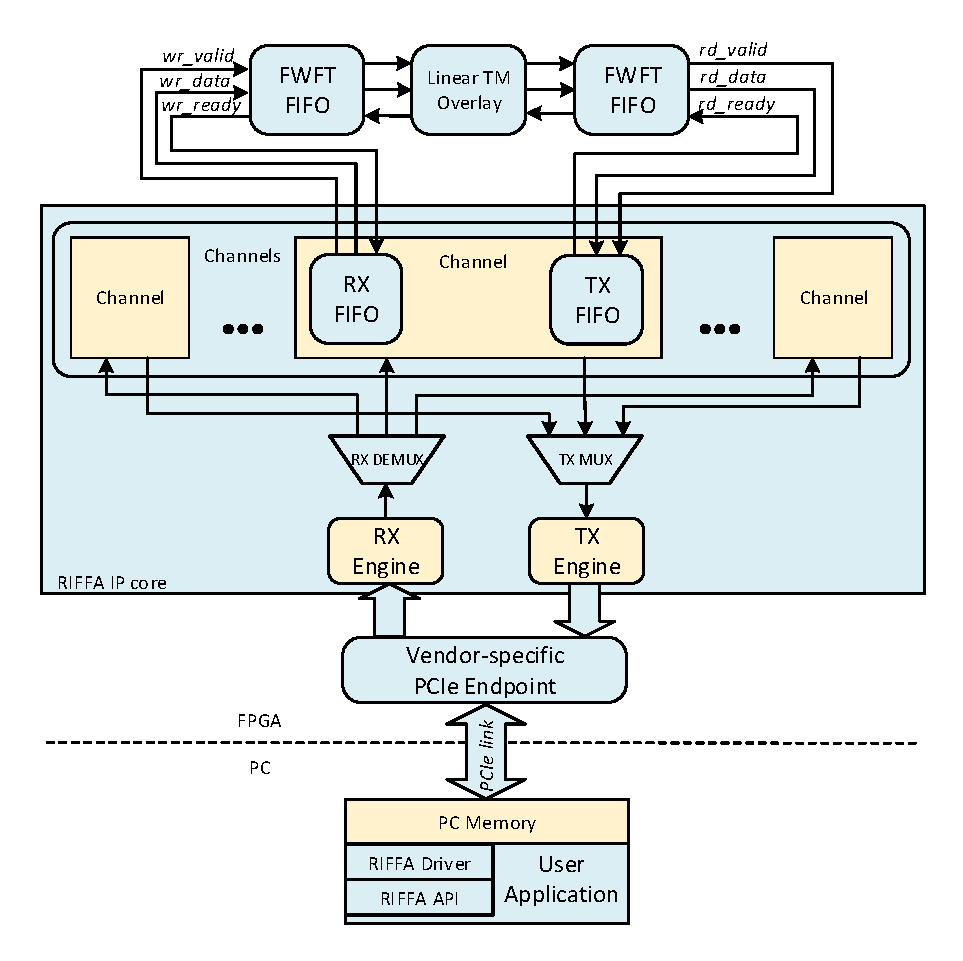
\includegraphics[width=0.9\columnwidth]{Figures/riffa.pdf}
%	\caption{RIFFA-based overlay accelerator.}
%	\label{riffa}
%\end{figure}


\subsection{Interfacing with DyRACT}
The original version of DyRACT communication infrastructure enables PCIe-based high-speed communication between a host computer and FPGA-based user logic with support for partial reconfiguration (PR). 
It provisions multiple AXI4-stream backend interface, enabling seamless integration with vendor-supported IP cores. 
We have modified the original version to make it lite-weight and tailored to support the proposed overlay architecture. 
Since the present implementation does not exploit PR, the reconfiguration control logic is disabled, and a single backend AXI4-stream interface is enabled. 
The stream interface width is configurable through width-conversion FIFOs. 
A new AXI-Lite interface is added to support command-data interface between the host and the overlay.
The software architecture follows similar structure of that of RIFFA. 
The low-level communication protocols and interrupts are managed by the driver and the user library provides APIs for integration with application programmes. 


\subsection{Programming Model}
%%%Emphasizing the importance of DyRACT%%%
While Xillybus and RIFFA provide RTL design along with the driver support and software code demos, they generally do not have direct access to the FPGA RAMs (Xillybus AXI version has limited access to the registers). 
In comparison, DyRACT offers simple register access via the AXI-Lite interface. 
Thus,  user can easily send the instructions and streaming data from the host PC to the FPGA at runtime using dedicated APIs, instead of reconfiguring the overlay. 
A user-friendly programming model is proposed for the linear TM overlay integrated with DyRACT system. 
There are three register files developed for overlay control purpose. 
One register file (0x30) is written with a 4-bit tag, which is followed by a register file (0x34) to restore the instruction with its corresponding FU. 
Another register file (0x38) is used to store the number of data words to be input to the first FU for a specific comptuter kernel (based on the instructions) and the value of (II-1), when the instruction load has been done. 
Afterwards, a bunch of user-defined data can be transferred to the FPGA, and will be sent back to the host PC after the processing of the overlay. 
A snippet example code shows how to load the instructions, setup the overlay, and write the data to the FPGA is presented in Table~\ref{program}. 

\lstset { %
	language=C,
	backgroundcolor=\color{white}, % set backgroundcolor
	%basicstyle=\footnotesize,% basic font setting
	%basicstyle=\ttfamily\tiny,
	basicstyle=\ttfamily\small,
	keywordstyle=\color{blue}\ttfamily,
	stringstyle=\color{blue}\ttfamily,
	commentstyle=\color{green}\ttfamily,
	breaklines=true	
}
\lstset{framesep=-10pt, xleftmargin=-10pt}

\begin{table}[!h]
	\centering
	\caption{Example code.}
	\label{program}
	\begin{tabular}{l}
		%    \toprule
		%		\multicolumn{1}{c}{(a) C description}  &\multicolumn{1}{c}{(b) DFG description} \\ % Assembly with Loopback Optimization
		%    \midrule
		%    \hspace{-0.2in}
		%    \hspace{-0.2in}
		\begin{lstlisting}
fpga_reg_wr(0x30,0x0); //Tag of FU0 
fpga_reg_wr(0x34,0x3033D080); // Instruction 0
		
fpga_reg_wr(0x30,0x1); //Tag of FU1
fpga_reg_wr(0x34,0x8852000); // Instruction 1
		
fpga_reg_wr(0x38,5); // No. of input data
fpga_reg_wr(0x38,5); // (II-1)
		
dyract_send_data((unsigned char *)mydata, sendSize*sizeof(int)); //Send data
dyract_recv_data((unsigned char *) recvdata, recvSize*sizeof(4)); //Receive data
		\end{lstlisting}\\
		%    \bottomrule
	\end{tabular}
\end{table}


The 32-bit instructions are written in hexadecimal style in Table~\ref{program}, which are used as configurations for the DSP-based FUs. 
A description of the instruction format, using \textit{ADD R3, R5 (WB)} operation as an example, is shown in Table~\ref{instruction}. 
From this table, it can be seen that a 32-bit instruction has four sections, the 18-bit ALU control, the 2-bit input map multiplexing, two 5-bit source operand addresses, with the remaining 2-bit reserved for future use. 
%At the end of the FU context write cycle, each FU contains the instructions that it needs to execute (in the IM) and the number of instructions that it needs to execute (in the IC register). 

\begin{table*}
	\renewcommand{\arraystretch}{1.2}
	\caption{Instruction format.}
	\label{instruction}
	\scriptsize
	\centering
	\resizebox{\textwidth}{!}{	
		\begin{tabular}{|c|c|c|c|c|c|c|c|c|c|c|c|c|c|}
			\hline
			FU part          &                         \multicolumn{8}{c|}{ALU Control}                         & \multicolumn{2}{c|}{Input Map Control} & \multicolumn{2}{c|}{RF Control} & Reserved \\ \hline
			Signals          & \textit{NDF} & \textit{WB} & alumode & inmode  & opmode  & cea2 & ceb2 & usemult & split &             immop              &  src1  &          src2          &          \\ \hline
			No. of bits        &      1       &      1      &    4    &    2    &    7    &  1   &  1   &    1    &   1   &               1                &   5    &           5            &    2     \\ \hline
			Locations         &     [30]     &    [29]     & [28:25] & [24:23] & [22:16] &  15  &  14  &   13    &  12   &               11               & [10:6] &         [5:1]          & [31][0]  \\ \hline
			ADD R3, R5 (\textit{WB}) &      0       &      1      &  0000   &   00    & 0110011 &  1   &  1   &    0    &   1   &               0                & 00011  &         00101          &   0 0    \\ \hline
	\end{tabular}}
\end{table*}


\section{Experimental Setup}
\label{section_5}
We conducted experiments for both the AXI bus-based and PCIe-based overlay accelerators.  
For the AXI bus-based system, the experimental software runs on the ARM processor of the Xilinx ZedBoard. 
For the PCIe-based accelerators (implemented using PCIe-Xillybus, RIFFA and DyRACT respectively), the experiments are run on an HP Z420 workstation (six 3.5 GHz Intel Xeon E5-1650 cores) with a Xilinx VC707 evaluation board plugged into the PCIe Gen2 slot of the motherboard. 

\subsection{AXI-Xillybus System}
The AXI-Xillybus system is using one 32-bit wide AXI ACP port for data transmission, running at a frequency of 100 MHz on the Xilinx ZedBoard. 
Hence the theoretical total bandwidth of this system is 800 MB/s, and the maximum streaming throughput is 400 MB/s in a full-duplex system. 

\subsubsection{AXI-Xillybus Loopback Test}
Before the accelerator system can be developed, we first ensure that the demonstration bundle provided by the Xillybus vendor operates correctly on our Zynq-based system. 
%The demonstration bundle includes an example FPGA design containing just a single FIFO used to loop the data back, along with a device driver and sample software code. 
We evaluate the performance of Xillybus by testing the round-trip data transmission throughput with the default settings, using sequential and parallel (multi-threading) programming for \textit{read} and \textit{write} functions respectively. 
%the write function and read function are executing sequentially by default, which means the read process has to wait until the write process has finished. 
%It is inefficient for a full-duplex interface to work in half-duplex mode, and so as to make full use of the Xillybus IP core, we adopt a multi-threading technique (using Pthreads) to improve its performance by creating two different threads for the write and read functions respectively. 

The bandwidth of the loopback test for AXI-Xillybus using different data block sizes is shown in Figure~\ref{axi_xillybus_loopback_bw}. 
As seen from this diagram, the single-threaded loopback test saturates at a throughput of around 150 MB/s (maximum of 160 MB/s) when the transfer size exceeds 8K words, while the multi-thread loopback test saturates (with a maximum throughput of 330 MB/s) when the transfer size exceeds 500K words. 
The two dashed lines indicate the theoretical throughput of the 32-bit AXI-ACP port running at 100 MHz.
The throughput of the multi-thread test surpasses that of the single-thread test for data block sizes exceeding 64K words, and for large block sizes achieves approximately twice the throughput. 
Creating Pthreads introduces a significant overhead for smaller transfer sizes, thus the multi-threading version is only applicable for large data transfers. 

\pgfplotsset{
	axis background/.style={fill=none},
	%tick style=mygrey2,
	%tick label style=mygrey2,
	grid=none,
	%xtick pos=left,
	%ytick pos=left,
	tick style={
		major grid style={style=white,line width=1pt},minor grid style=white,
%		major grid style={style=white,line width=1pt},minor grid style=mygrey3,
		%tick align=outside,
	},
	%minor tick num=4,
}

\begin{figure}[tb]
	\centering
	 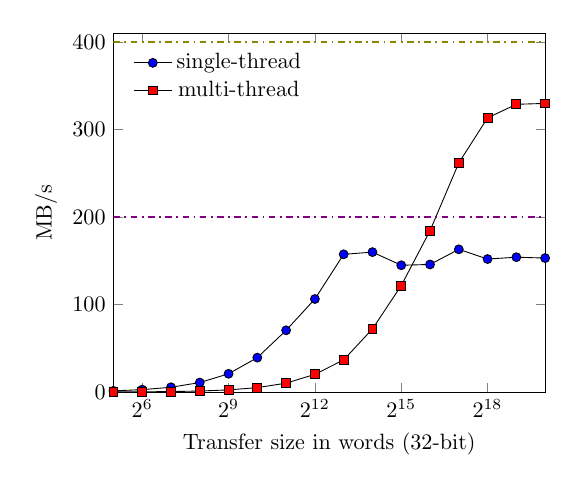
\begin{tikzpicture}[scale = 0.8]
	 \begin{axis}[
	 xmode=log,
	 log basis x={2},
	 xlabel=Transfer size in words (32-bit),
	 ymin=0,
	 ymax=410,
	 xmax = 1048576,
	 xmin = 32,
	 ylabel=MB/s,
%	 legend style={at={(0.3,0.8)},anchor=north}
	 legend pos=north west,
	 legend style={draw=none}
	 ]    

	\addplot [mark=*,mark options={fill=blue}] plot coordinates {
		(32,     1.4)
		(64,     2.8)
		(128,     5.5)
		(256,     10.9)
		(512,      20.9)
		(1024,     39.4)
		(2048,     70.6)
		(4096,     106.4)
		(8192,     157.5)
		(16384,    160.0)
		(32768,    145.0)
		(65536,    145.9)
		(131072,    163.2)
		(262144,    152.1)
		(524288,    154.2)
		(1048576,    153.2)	
	}; 
	 \addplot [mark=square*,mark options={fill=red}] plot coordinates {
	 	(32,     0.2)
	 	(64,     0.3)
	 	(128,     0.6)
	 	(256,     1.2)
	 	(512,     2.5)
	 	(1024,     5.1)
	 	(2048,     10.2)
	 	(4096,     20.3)
	 	(8192,      36.8)
	 	(16384,     72.2)
	 	(32768,    121.7)
	 	(65536,    184.5)
	 	(131072,    262)
	 	(262144,    313.5)
	 	(524288,    329)
	 	(1048576,    330)
	 }; 
	 \addplot [color=violet,thick,dash dot] plot coordinates {
	 	(32,     200)
		(64,     200)
		(128,     200)
		(256,     200)
		(512,     200)
		(1024,     200)
		(2048,     200)
		(4096,     200)
		(8192,     200)
		(16384,    200)
		(32768,    200)
		(65536,    200)
		(131072,    200)
		(262144,    200)
		(524288,    200)
		(1048576,   200)	
	 };

	 \addplot [color=olive,thick,dash dot] plot coordinates {
	(32,     400)
	(64,     400)
	(128,     400)
	(256,     400)
	(512,     400)
	(1024,     400)
	(2048,     400)
	(4096,     400)
	(8192,     400)
	(16384,    400)
	(32768,    400)
	(65536,    400)
	(131072,   400)
	(262144,   400)
	(524288,   400)
	(1048576,  400)	
};

	 \legend{single-thread\\multi-thread\\}
	 \end{axis}
	 \end{tikzpicture}	
	
	\caption[]{AXI-Xillybus loopback test evaluation.} 
	\label{axi_xillybus_loopback_bw}
	
\end{figure}


\subsubsection{AXI-Xillybus based Overlay Accelerator}
Xillybus provides an online IP core factory for users to customize the interface on demands.
%The accelerator and its data streams are shown in Figure~\ref{axi_xillybus_overlay}. 
In our design, two 32-bit streaming device files are instantiated for data acquisition and one 32-bit seekable device file is responsible for the instruction load and overlay setup. 
We evaluate the performance of the overlay accelerator which is an integration of the linear TM overlay as discussed in Section~\ref{section_3} and AXI-Xillybus interface, and compare to VectorBlox MXP~\cite{severance2013embedded}, in terms of bandwidth and area consumption. 
To perform this comparison, we use the set of kernels shown in Table~\ref{benchmarks_system}, which are extracted from compute intensive applications available from~\cite{gopalakrishnan2007finding, hoy2015performance}. 
Both the overlay accelerator and MXP are running on Xillinux-2.0, which is the latest Linux distribution released for ZedBoard (kernel 4.4), with AXI-Xillybus using the Pthread multi-threading technique with a data block transfer size of 1M words.

\begin{table}[tb]
%	\renewcommand{\arraystretch}{1.2}
	\caption{DFG characteristics of benchmark set.}
	\label{benchmarks_system}
	\centering
	\resizebox{\columnwidth}{!}{
	\begin{tabular}{clccccc}
		\toprule
		\multirow{3}{*}{No.} & \multirow{3}{*}{Benchmark} &  \multicolumn{5}{c}{Characteristics}  \\ \cline{3-7}
		                     &                            &  I/O  & graph &  op   & graph & graph \\
		                     &                            & nodes & edges & nodes & depth & width \\ \midrule
		         1.          & chebyshev                  &  1/1  &  12   &   7   &   7   &   1   \\
		         2.          & mibench                    &  3/1  &  22   &  13   &   6   &   3   \\
		         3.          & qspline                    &  7/1  &  50   &  25   &   8   &   6   \\
		         4.          & fft                        &  6/4  &  24   &  10   &   3   &   4   \\
		         5.          & kmeans                     & 16/1  &  39   &  23   &   5   &   8   \\
		         6.          & mm                         & 16/1  &  31   &  15   &   4   &   8   \\
		         7.          & spmv                       & 16/2  &  30   &  14   &   4   &   8   \\
		         8.          & stencil                    & 15/2  &  30   &  14   &   5   &   6   \\ \bottomrule
	\end{tabular}
	}
\end{table}

Figure~\ref{axi_xillybus_mxp_bw} shows the performance of a single 32-bit linear TM overlay (AXI-Xillybus-Overlay) and a 16-lane 32-bit MXP (MXP-V16) implemented on a ZedBoard for the benchmarks given in Table~\ref{benchmarks_system}. 
As seen from the figure, MXP-V16 outperforms AXI-Xillybus-Overlay over all benchmarks (with the exception of `chebyshev'). 
Table~\ref{xillybus_mxp_area} shows the hardware resource usage of the AXI-Xillybus based overlay accelerator and MXP-V16. 
As seen from this table, AXI-Xillybus-Overlay is much more area efficient, and consumes only 19.8\% LUTs, 26.1\% FFs, 7.6\% BRAMs and 7.1\% DSP blocks, compared to MXP-V16. 

\pgfplotsset{
	axis background/.style={fill=white},
	tick style=black,
	tick label style=black,
	grid=both,
	xtick pos=left,
	ytick pos=left,
	tick style={
		major grid style={style=white,line width=1pt},minor grid style=white,
		tick align=outside,
	},
	minor tick num=4,
}

\begin{figure}[tb]
	\centering
	\pgfplotstableread{
		0		379.7	342		217		195.4
		1		245.7	317		226.7	292.6
		2		203.1	422		227.5	472.6
		3		94		158.7	225.6	380.9
		4		83.9	207.9	233.5	578.5
		5		53.9	142		229.9	605.9
		6		49.7	127.9	227.1	584.7
		7		52.7	134		225.8	574.3
	}\datathroughput	
%	\pgfplotstableread{
%		0		379.7	342		434		390
%		1		237		317		292		390
%		2		191.4	422		245		540
%		3		94		158.7	376		635
%		4		77.8	207.9	230		942
%		5		51.4	142		233		644
%		6		47.2	127.9	243		658
%		7		50.6	134		246		651
%	}\datathroughput
	\subfigure[Data processing throughput in MB/s]{
		\begin{tikzpicture}[scale = 0.9]
		\centering
		\begin{axis}[
%		axis y line=left,
		ybar=0pt,
		width=17cm,
		x = 0.85cm,
		height=5.3cm,
		ymin=0,
		ymax=1000,        
		ylabel={MB/s},
		grid style={dotted,gray},
		ymajorgrids=true,
		%	nodes near coords,    
		xtick=data,
		bar width = 5, %0.2
		xticklabels = {
			\strut chebyshev,
			\strut mibench,
			\strut qspline,
			\strut fft,
			\strut kmeans,
			\strut mm,
			\strut spmv,
			\strut stencil                                     
		},
		x tick label style={rotate=45, anchor=north east, inner sep=0mm},
		major x tick style = {opacity=0},
		minor x tick num = 1,
		minor tick length=1ex,
		%	every node near coord/.append style={
		%		anchor=west,
		%		rotate=90,
		%		font=\tiny
		%	},
		]
		
		\addplot[draw=black,fill=blue, draw opacity=1] table[x index=0,y index=3] \datathroughput;\label{MB_xillybus_axi}
		\addplot[draw=black,fill=red, draw opacity=1] table[x index=0,y index=4]   \datathroughput;\label{MB_mxp} 					
		\end{axis}
		
		\node [draw=none, fill=white] at (rel axis cs: 0.4, 0.8) {\shortstack[l]{
				\ref{MB_xillybus_axi} AXI-Xillybus-Overlay \\ \ref{MB_mxp} MXP-V16 }};	
		\end{tikzpicture}
	}

	\subfigure[Throughput in MOPS]{
		\begin{tikzpicture}[scale = 0.9]
		\centering
		\begin{axis}[
%		axis y line=right,
		ybar=0pt,
		width=17cm,
		x = 0.85cm,
		height=5.3cm,
		ymin=0,
		ymax=800,        
		ylabel={MOPS},
		grid style={dotted,gray},
		ymajorgrids=true,
		%	nodes near coords,    
		xtick=data,
		bar width = 5, %0.2
		xticklabels = {
			\strut chebyshev,
			\strut mibench,
			\strut qspline,
			\strut fft,
			\strut kmeans,
			\strut mm,
			\strut spmv,
			\strut stencil                                   
		},
		x tick label style={rotate=45, anchor=north east, inner sep=0mm},
		major x tick style = {opacity=0},
		minor x tick num = 1,
		minor tick length=1ex,
		%	every node near coord/.append style={
		%		anchor=west,
		%		rotate=90,
		%		font=\tiny
		%	},
		]
		
		\addplot[draw=black,fill=blue, draw opacity=1] table[x index=0,y index=1] \datathroughput;\label{MOPS_xillybus_axi}
		\addplot[draw=black,fill=red, draw opacity=1] table[x index=0,y index=2]   \datathroughput;\label{MOPS_mxp} 					
		\end{axis}
		
		\node [draw=none, fill=white] at (rel axis cs: 0.4, 0.8) {\shortstack[l]{
				\ref{MOPS_xillybus_axi} AXI-Xillybus-Overlay \\ \ref{MOPS_mxp} MXP-V16 }};	
		\end{tikzpicture}
	}
	
	\caption{Performance comparison for the benchmarks using a transfer size of 1M words.}
	\label{axi_xillybus_mxp_bw}
\end{figure}

The MXP memory system is based on one 64-bit AXI HP port running at a frequency of 110 MHz while AXI-Xillybus is based on a single 32-bit AXI ACP port running at a frequency of 100 MHz. 
This corresponds to a theoretical maximum throughput of 880 MB/s for MXP-V16 and 400 MB/s for AXI-Xillybus-Overlay. 
As seen from Figure~\ref{axi_xillybus_mxp_bw}, MXP-V16 achieves a throughput of 460.6 MB/s (52.3\% of theoretical maximum) on average while AXI-Xillybus has a throughput of 226.6 MB/s (56.6\% of theoretical maximum) on average. 
%Figure~\ref{axi_xillybus_mxp_bw} indicates that AXI-Xillybus-V3 has a worse performance for the benchmarks with a larger number of I/O nodes. 
The throughput of AXI-Xillybus is about half of that of MXP-V16, mainly due to AXI-Xillybus using only 32-bit of the available 64-bit ACP port while MXP-V16 uses the full 64-bit HP port. 


\begin{table}[tb]
%	\renewcommand{\arraystretch}{1.2}
	\caption{Area overhead of AXI bus-based systems.}
	\label{xillybus_mxp_area}
	\centering
	\resizebox{\columnwidth}{!}{
	\begin{tabular}{lrrrr}
		\toprule
		\multirow{2}{*}{System} &                \multicolumn{4}{c}{Resource Usage}                \\ \cline{2-5}
		                        &            LUTs &              FFs &        BRAMs &         DSPs \\ \midrule
		Overlay                 &           1,747 &            1,954 &            0 &            8 \\
		AXI-Xillybus            &           4,000 &            3,844 &            5 &            0 \\ \midrule
		MXP-V16                 &          28,974 &           22,174 &           66 &          112 \\ \midrule
		\textbf{Available}      & \textbf{53,200} & \textbf{106,400} & \textbf{140} & \textbf{220} \\ \bottomrule
	\end{tabular}
	}
\end{table}

Although the AXI bus-based Xillybus provides an area efficient interface solution for the Xilinx Zynq SoC, the throughput is still far below the theoretical maximum shown in Table~\ref{theo_bw}. 
This is mainly due to not making good use of the available HP/ACP ports (Xillybus uses only one 32-bit port which is operating at a frequency of 66.7\% of the theoretical maximum that the AXI bus on Zynq can support). 


\subsection{PCIe System}
Our PCIe system is based on the Gen2$\times$8 PCIe interface running at a frequency of 250 MHz on the Xilinx VC707 platform, which corresponds to a maximum bandwidth of 8000 MB/s and hence a maximum streaming throughput of 4000 MB/s for a full-duplex system. 


\subsubsection{Loopback Test}
%%% Combine Xillybus, RIFFA and DyRACT together %%%

\subsubsection{PCIe-Xillybus Loopback Test}
Xillybus has been upgraded to a new version (PCIe-Xillybus) to support high performance PCIe interface communication since 2015. 
The block diagram of PCIe-Xillybus for data loopback is almost the same as that of AXI-Xillybus, except that the 32-bit FIFO is replaced with a 128-bit FIFO and the Xillybus hardware module \textit{Xillybus.v} (including the Xillybus IP core and a Xilinx 7 series integrated block for PCIe) is connected to an HP Z420 workstation via the PCIe link. 
Similar to AXI-Xillybus, we developed two host programs to evaluate the round-trip bandwidth in both half-duplex and full-duplex mode. 

The bandwidth of the loopback test for PCIe-Xillybus using different data block sizes is shown in Figure~\ref{pcie_xillybus_riffa_loopback_bw}. 
As seen from this diagram, the data transmission is very slow when the transfer size is less than 32K words. 
This is due to large system overhead for a data buffer size of less than 128 KBytes~\cite{xillybus2018}. 
The single-threaded loopback test saturates at a throughput of 1900 MB/s when the transfer size exceeds 128K words, while the multi-thread loopback test saturates (with a maximum throughput of 2300 MB/s) when the transfer size exceeds 500K words. 
%The single-threaded loopback test saturates at a throughput of around 1900 MB/s (maximum of 2000 MB/s) when the transfer size exceeds 128K words, while the multi-thread loopback test saturates (with a maximum throughput of 2300 MB/s) when the transfer size exceeds 500K words. 
The two dashed lines indicate the theoretical bandwidth of the Gen2$\times$8 PCIe interface running at 250 MHz.
The throughput of the multi-thread test surpasses that of the single-thread test for data block sizes exceeding 256K words, and achieves around 1.2$\times$ higher bandwidth when transferring 1M words. 
Although the throughput of the multi-thread test is not as expected (twice that of the single-thread test), it shows better performance for the transmission of large data blocks. 

%\pgfdeclarelayer{background}
%\pgfdeclarelayer{foreground}
%\pgfsetlayers{background,main,foreground}

\pgfplotsset{
	axis background/.style={fill=none},
	%tick style=mygrey2,
	%tick label style=mygrey2,
	grid=none,
	%xtick pos=left,
	%ytick pos=left,
	tick style={
		major grid style={style=white,line width=1pt},minor grid style=white,
%		major grid style={style=white,line width=1pt},minor grid style=mygrey3,
		%tick align=outside,
	},
	%minor tick num=4,
}

\begin{figure}[tb]
	\centering
	 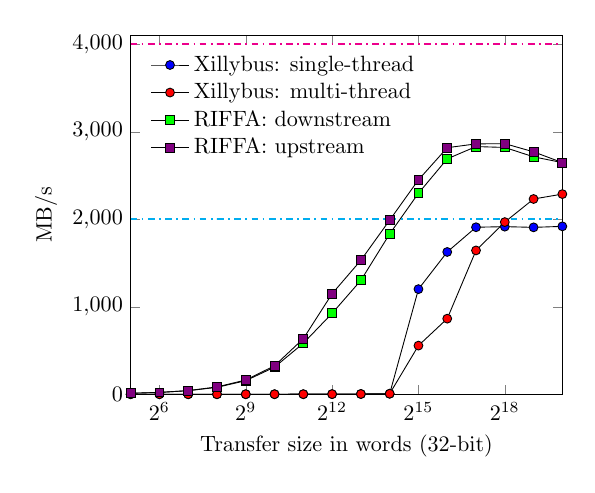
\begin{tikzpicture}[scale = 0.8]
	 \begin{axis}[
	 xmode=log,
	 log basis x={2},
	 xlabel=Transfer size in words (32-bit),
	 ymin=0,
	 ymax=4100,
	 xmax = 1048576,
	 xmin = 32,
	 ylabel=MB/s,
%	 legend style={at={(0.3,0.8)},anchor=north}
	 legend cell align={left},
	 legend pos=north west,
	 legend style={draw=none}
	 ]    

	\addplot [mark=*,mark options={fill=blue}] plot coordinates {
		(32,     0)
		(64,     0)
		(128,    0.05)
		(256,     0.1)
		(512,      0.2)
		(1024,     0.35)
		(2048,     0.7)
		(4096,     1.45)
		(8192,     2.9)
		(16384,    5.85)
		(32768,    1201.5)
		(65536,    1626.5)
		(131072,   1909.1)
		(262144,   1915.8)
		(524288,   1907.7)
		(1048576,  1919.1)	
	}; 
	 \addplot [mark=*,mark options={fill=red}] plot coordinates {
	 	(32,     0)
	 	(64,     0)
	 	(128,    0.04)
	 	(256,    0.08)
	 	(512,    0.16)
	 	(1024,   0.32)
	 	(2048,   0.68)
	 	(4096,   1.36)
	 	(8192,   2.76)
	 	(16384,  5.85)
	 	(32768,  556)
	 	(65536,  864)
	 	(131072, 1644)
	 	(262144, 1968)
	 	(524288, 2232)
	 	(1048576, 2288)
	 }; 
	 
	 \addplot [mark=square*,mark options={fill=green}] plot coordinates {
	 	(32,     11.1)
	 	(64,     20.3)
	 	(128,    41.0)
	 	(256,    78.8)
	 	(512,    155.0)
	 	(1024,   310.0)
	 	(2048,   583.0)
	 	(4096,   924.6)
	 	(8192,   1302.1)
	 	(16384,  1832.8)
	 	(32768,  2297.8)
	 	(65536,  2691.1)
	 	(131072, 2831.3)
	 	(262144, 2821.2)
	 	(524288, 2713.9)
	 	(1048576,2647.7)	
	 }; 
	 \addplot [mark=square*,mark options={fill=violet}] plot coordinates {
	 	(32,     11.1)
	 	(64,     21.0)
	 	(128,    41.4)
	 	(256,    83.5)
	 	(512,    162.8)
	 	(1024,   325.5)
	 	(2048,   635.2)
	 	(4096,   1148.9)
	 	(8192,   1531.9)
	 	(16384,  1990.4)
	 	(32768,  2451.0)
	 	(65536,  2818.5)
	 	(131072, 2862.0)
	 	(262144, 2864.5)
	 	(524288, 2771.1)
	 	(1048576,2647.7)
	 }; 
	 
	 \addplot [color=cyan,thick,dash dot] plot coordinates {
	 	(32,     2000)
		(64,     2000)
		(128,     2000)
		(256,     2000)
		(512,     2000)
		(1024,     2000)
		(2048,     2000)
		(4096,     2000)
		(8192,     2000)
		(16384,    2000)
		(32768,    2000)
		(65536,    2000)
		(131072,    2000)
		(262144,    2000)
		(524288,    2000)
		(1048576,   2000)	
	 };

	 \addplot [color=magenta,thick,dash dot] plot coordinates {
		(32,     4000)
		(64,     4000)
		(128,     4000)
		(256,     4000)
		(512,     4000)
		(1024,     4000)
		(2048,     4000)
		(4096,     4000)
		(8192,     4000)
		(16384,    4000)
		(32768,    4000)
		(65536,    4000)
		(131072,   4000)
		(262144,   4000)
		(524288,   4000)
		(1048576,  4000)	
};
	
	\legend{Xillybus: single-thread\\Xillybus: multi-thread\\RIFFA: downstream\\RIFFA: upstream\\}
	\end{axis}
	\end{tikzpicture} 
%	\label{riffa_loopback_bw}
%	}
	
	\caption[]{PCIe system loopback test evaluation.} 
	\label{pcie_xillybus_riffa_loopback_bw}
	
\end{figure}


\subsubsection{RIFFA Loopback Test}
Similarly, a loopback design using RIFFA framework was also implemented. 
A first word fall through (FWFT) FIFO is used for data loop back, and the RIFFA IP core is acting as the bridge between the vendor-specific PCIe Endpoint and the FWFT FIFO. 
Data transmission is under the control of a finite state machine (FSM), which executes the upstream transfers and downstream transfers in different processing states.  
Thus, it is not possible to achieve full-duplex data transmission. 

The bandwidth for RIFFA data loopback is shown in Figure~\ref{pcie_xillybus_riffa_loopback_bw}. 
As seen from this diagram, both the upstream transfers (read) and downstream transfers (write) saturate at around 2.85 GB/s when the transfer size is equal to 128K sample words, corresponding a total bandwidth of 2.85 GB/s, as read and write cannot happen simultaneously. 
The bandwidth degrades slightly when the transfer size exceeds 128k words due to the overutilization of BRAMs.
As mentioned previously, the RIFFA hardware was not developed for full-duplex data transmission. 
Hence the send function (\textit{fpga\_send}) and receive function (\textit{fpga\_recv}) will execute sequentially and it is useless to use multi-threading techniques as was done for Xillybus. 

\subsubsection{DyRACT Loopback Test}
%%%%Description of DyRACT loopback test.%%%%
The bandwidth of the loopback test for DyRACT data loopback is shown in Figure~\ref{pcie_xillybus_riffa_loopback_bw}. 

%%%%Analysis of DyRACT loopback test.%%%%


\subsubsection{PCIe-Xillybus based Overlay Accelerator}
%Figure~\ref{pcie_xillybus_overlay} shows the PCIe-Xillybus based overlay accelerator and its data streams. 
In the PCIe-Xillybus based overlay accelerator system, we propose replicating four 32-bit linear TM overlays, interfacing with the 128-bit standard FIFOs to make full use of the data width.
Thus, two 128-bit streaming device files are instantiated for data acquisition and one 128-bit seekable device file is responsible for instruction load and overlay setup. 

\subsubsection{RIFFA based Overlay Accelerator}
Integration of the linear TM overlay with RIFFA is quite similar to that of Xillybus, except that the standard FIFOs are replaced with FWFT FIFOs.  
Although RIFFA has no access to the FPGA RAMs directly, it is possible to load the instructions and registers by adding a new state to the FSM control. 
The RX (view from the integrated overlay side) is divided into two processes: one for overlay initialization, and the other one for data transmission. 

\subsubsection{DyRACT based Overlay Accelerator}
%%%%Description of DyRACT based Overlay Accelerator.%%%%
Similarly, DyRACT is connected to four 32-bit linear TM overlays using two 128-bit standard FIFOs to buffer the data. 
We customise three memory arrays to save the instructions along with their tags to the FUs, and the number of input data or the value of II minus one. 

Figure~\ref{pcie_xillybus_riffa_bw} shows the performance of four 32-bit linear TM overlays integrated with PCIe-Xillybus (PCIe-Xillybus-Overlay), RIFFA (RIFFA-Overlay) and DyRACT (DyRACT-Overlay), respectively. 
PCIe-Xillybus-Overlay uses a block size of 1M words with the Pthread multi-threading technique, while RIFFA-Overlay and DyRACT-Overlay use a block size of 128K words.
All these overlay accelerators are running on an Ubuntu 14.04.5 workstation (six 3.5 GHz Intel Xeon E5-1650 cores) with a Xilinx VC707 evaluation board plugged into the PCIe Gen2 slot of the motherboard. 
As can be seen from Figure~\ref{pcie_xillybus_riffa_bw}, DyRACT-Overlay achieves an average throughput of 1540 MB/s (38.5\% of theoretical maximum), which is around 18\% higher than RIFFA-Overlay with an average throughput of 1300 MB/s and 4.3$\times$ better than PCIe-Xillybus-Overlay with an average throughput of 358 MB/s (9\% of theoretical maximum). 
The ratio of the throughput in Mega-operations per second (MOPS) is proportional to that of data processing throughput in MB/s. 
DyRACT-Overlay proves to be the best accelerator in terms of throughput. 
%%%%Add some analysis%%%%

\pgfplotsset{
	axis background/.style={fill=white},
	tick style=black,
	tick label style=black,
	grid=both,
	xtick pos=left,
	ytick pos=left,
	tick style={
		major grid style={style=white,line width=1pt},minor grid style=white,
		tick align=outside,
	},
	minor tick num=4,
	compat = 1.3,
}

\begin{figure}[tb]
	\centering
	\pgfplotstableread{
		0		677		1448	2081	386.9		828		 1190
		1		381		1469	1680	351.5		1355	 1550
		2		312		1250	1657	349.5		1400	 1856
		3		155		582		683		372			1396	 1640
		4		127		494		578		353.4		1375	 1610
		5		83		321		324		354			1369	 1383
		6		76		300		328		347.3		1370	 1496
		7		82		310		370		351.3		1328	 1587
	}\datathroughput	
	\subfigure[Data processing throughput in MB/s]{
		\begin{tikzpicture}[scale = 0.9]
		\centering
		\begin{axis}[
%		axis y line=left,
		ybar=0pt,
		width=17cm,
		x = 0.85cm,
		height=5.3cm,
		ymin=0,
		ymax=3000,        
		ylabel={MB/s},
		grid style={dotted,gray},
		ymajorgrids=true,
		%	nodes near coords,    
		xtick=data,
		bar width = 5, %0.15
		xticklabels = {
			\strut chebyshev,
			\strut mibench,
			\strut qspline,
			\strut fft,
			\strut kmeans,
			\strut mm,
			\strut spmv,
			\strut stencil                                     
		},
		x tick label style={rotate=45, anchor=north east, inner sep=0mm},
		major x tick style = {opacity=0},
		minor x tick num = 1,
		minor tick length=1ex,
		%	every node near coord/.append style={
		%		anchor=west,
		%		rotate=90,
		%		font=\tiny
		%	},
		]
		
		\addplot[draw=black,fill=blue, draw opacity=1] table[x index=0,y index=4] \datathroughput;\label{MB_xillybus_pcie}
		\addplot[draw=black,fill=red, draw opacity=1] table[x index=0,y index=5]   \datathroughput;\label{MB_riffa} 
		\addplot[draw=black,fill=green, draw opacity=1] table[x index=0,y index=6]   \datathroughput;\label{MB_dyract} 						
		\end{axis}
		
		\node [draw=none, fill=white, font=\small] at (rel axis cs: 0.6, 0.8) {\shortstack[l]{
				\ref{MB_xillybus_pcie} PCIe-Xillybus-Overlay  \ref{MB_riffa} RIFFA-Overlay \\ \ref{MB_dyract} DyRACT-Overlay }};	
		\end{tikzpicture}
	}

	\subfigure[Throughput in MOPS]{
		\begin{tikzpicture}[scale = 0.9]
		\centering
		\begin{axis}[
%		axis y line=right,
		ybar=0pt,
		width=17cm,
		x = 0.85cm,
		height=5.3cm,
		ymin=0,
		ymax=3300,        
		ylabel={MOPS},
		grid style={dotted,gray},
		ymajorgrids=true,
		%	nodes near coords,    
		xtick=data,
		bar width = 5, %0.15
		xticklabels = {
			\strut chebyshev,
			\strut mibench,
			\strut qspline,
			\strut fft,
			\strut kmeans,
			\strut mm,
			\strut spmv,
			\strut stencil                                      
		},
		x tick label style={rotate=45, anchor=north east, inner sep=0mm},
		major x tick style = {opacity=0},
		minor x tick num = 1,
		minor tick length=1ex,
		%	every node near coord/.append style={
		%		anchor=west,
		%		rotate=90,
		%		font=\tiny
		%	},
		]
		
		\addplot[draw=black,fill=blue, draw opacity=1] table[x index=0,y index=1] \datathroughput;\label{MOPS_xillybus_pcie}
		\addplot[draw=black,fill=red, draw opacity=1] table[x index=0,y index=2]   \datathroughput;\label{MOPS_riffa} 	
		\addplot[draw=black,fill=green, draw opacity=1] table[x index=0,y index=3]   \datathroughput;\label{MOPS_dyract} 					
		\end{axis}
		
		\node [draw=none, fill=white, font=\small] at (rel axis cs: 0.6, 0.8) {\shortstack[l]{
				\ref{MOPS_xillybus_pcie} PCIe-Xillybus-Overlay  \ref{MOPS_riffa} RIFFA-Overlay \\ \ref{MOPS_dyract} DyRACT-Overlay }};	
		\end{tikzpicture}
	}
	
	\caption{Performance comparison for the benchmarks.}
	\label{pcie_xillybus_riffa_bw}
\end{figure}

Table~\ref{pcie_xillybus_riffa_area} shows a breakdown of the FPGA resource usage of the overlay, PCIe-Xillybus, RIFFA and DyRACT. 
%RIFFA-Overlay consumes 15\% fewer LUTs, 49\% more FFs, 29$\times$ more BRAMs and the same DSP blocks compared to PCIe-Xillybus-Overlay. 
PCIe-Xillybus-Overlay consumes least number of FFs (33\% fewer than RIFFA-Overlay), while RIFFA-Overlay costs least number of LUTs (21\% fewer than DyRACT-Overlay) and DyRACT-Overlay is most area efficient in BRAMs consumption (96\% fewer than RIFFA-Overlay). 
While the logic and DSP resources used are comparable among all these implementations, there is a big difference in the BRAM utilization specifically for RIFFA-Overlay.
This is due to the half-duplex mode of the RIFFA interface, resulting in a significant BRAM consumption to implement the two large depth FWFT FIFOs. 
Developing a full-duplex RIFFA based system would minimize the BRAM resource usage. 
At current stage, DyRACT-Overlay and PCIe-Xillybus-Overlay are much better than RIFFA-Overlay in terms of area efficiency. 
 
\begin{table}[tb]
%	\renewcommand{\arraystretch}{1.2}
	\caption{Area overhead of PCIe-based systems.}
	\label{pcie_xillybus_riffa_area}
	\centering
	\resizebox{\columnwidth}{!}{
	\begin{tabular}{lrrrr}
		\toprule
		\multirow{2}{*}{System} &                  \multicolumn{4}{c}{Resource Usage}                   \\ \cline{2-5}
		                        &             LUTs &              FFs &          BRAMs &           DSPs \\ \midrule
		Overlay                 &            6,988 &            7,816 &              0 &             32 \\
		PCIe-Xillybus           &            9,039 &            4,672 &           14.5 &              0 \\
		RIFFA                   &            6,669 &           10,765 &          289.5 &              0 \\
		DyRACT                  &           10,356 &            8,648 &             10 &              0 \\
		\textbf{Available}      & \textbf{303,600} & \textbf{607,200} & \textbf{1,030} & \textbf{2,800} \\ \bottomrule
	\end{tabular}
	}
\end{table}

%%\section{Discussion}
%We saw that AXI-Xillybus-V3 represents a very area efficient implementation compared with VectorBlox MXP-V16, at the expense of around half of the throughput. However,  AXI-Xillybus has only half the theoretical bandwidth of MXP, as Xillybus uses just 32-bits of an ACP port while MXP uses the full 64-bits of an HP port. If Xillybus were modified to use a 64-bit port (something that will be left for future work), and two parallel V3 overlays were implemented, both implementations would then have similar throughput. The AXI-Xillybus dual V3 implementation would require significantly fewer hardware resources (approximately 20\% of the LUTS and 8\% of the hard macros (BRAM and DSP) required by MXP on Zynq. Thus, the linear TM overlay represents a relatively efficient implementation when FPGA resources are limited, as would be the case when an accelerator was used with other major subsystems in a design.


%PCIe-Xillybus-V3 and RIFFA-V3 are proposed for more high-performance centric accelerator systems. The PCIe-Xillybus-V3 has a 1.6$\times$ better performance compared to the AXI-Xillybus-V3, at the expense of more than twice of resource consumption. However, the throughput of PCIe-Xillybus-V3 is slightly less than that of MXP-V16, as it achieves only 9\% of the theoretical maximum of the PCIe Gen2x8 interface. Among all the 4 implementations, RIFFA-V3 shows the best performance, with a throughput of 1300 MB/s on average. However, the half-duplex mode of RIFFA-V3 results in an over-utilization of BRAMs.

\section{Discussion and Conclusions}
In this paper, we have proposed overlay accelerator systems based on two different memory interfaces, AXI and PCIe. 
The AXI-Xillybus-Overlay represents a very area efficient implementation compared with VectorBlox MXP-V16, but with about half of the throughput. 
AXI-Xillybus has only half the theoretical bandwidth of MXP, as Xillybus uses just 32-bits of an ACP port while MXP uses the full 64-bits of an HP port. 
If Xillybus were modified to use a 64-bit ACP port and two parallel V3 overlays were implemented, it would achieve a throughput close to MXP-V16, but with significantly fewer hardware resources (approximately 20\% of the LUTS and 8\% of the hard macros (BRAM and DSP) required by MXP on Zynq.
Thus, the linear TM overlay represents a relatively efficient implementation when FPGA resources are limited, as would be the case when an accelerator was used with other major subsystems in an FPGA based SoC design.

The PCIe-Xillybus-Overlay, RIFFA-Overlay and DyRACT-Overlay were also proposed for more high-performance centric accelerator systems. 
The DyRACT-Overlay has a 4.3$\times$ speed improvement when compared to the PCIe-Xillybus-Overlay, and a 6.8$\times$ better throughput than the AXI-Xillybus-Overlay, achieving a throughput of 1540 MB/s on average. 
Both DyRACT-Overlay and RIFFA-Overlay appear to be promising overlay accelerator for high computing purposes, however, there is a need to develop a full-duplex system for RIFFA-Overlay, which will not only reduce its BRAM utilization, but also potentially improve the throughput with parallel programming method. 

We open source the DyRACT-Overlay framework for future research and it can be downloaded from https://github.com/louislxw/linear\_tm\_overlay. 

\section*{Acknowledgment}

This work is supported by the Singapore Ministry of Education (MOE) Academic Research Fund Tier 2 under grant MOE2017-T2-1-002.

\def\IEEEbibitemsep{1pt plus 1pt}
%\footnotesize
%\scriptsize
\bibliographystyle{abbrv}
% argument is your BibTeX string definitions and bibliography database(s)
\bibliography{Files/references}


\end{document}
